\section{Introduction}
This chapter presents feasibility study and planning, power balancing and control mechanisms, and battery energy storage systems. Additionally, model development of the DC microgrid and a discussion on the state chart model for the Energy Management System (EMS) are provided. By systematically examining these aspects, the objective is to establish the grid structure to be utilized in the simulation.\par
\section{Feasibility study and planning}
The objective of this study is to implement an energy management system in a DC microgrid with the aim of enhancing overall system performance. The feasibility studies for the EMS are closely reliant on the feasibility study of the DC microgrid, given that they constitute an addition to the DC microgrid. The feasibility of DC MG is studied in this chapter. \par
The viability of DC MG in residential areas is evaluated in comparison to the ac grid in terms of conversion efficiencies in \cite{33}. The author concluded that DC systems with local generation and storage encounter less conversion losses, this was supported by \cite{34}, they developed AC and DC models for comparison  and concluded that when AC power system is supplied by a DC source, further losses can be expected resulting in further benefits of a DC distribution system. The highest efficiency is attained when DC sources supply DC loads, and AC sources supply AC loads. The positive outcome demonstrated in \cite{35} has established the feasibility of directly supplying appliances with DC voltage.\par
\section{Resource Assessment and Design}
\subsection{Battery Energy Storage System}
The battery SOC level determines the duration of use of electrical energy after sunset \cite{36} and if the battery capacity is too low the grid is likely to shut down. For the EMS to effectively keep the grid stable the SoC of the battery must always be known. The charging/discharging effect on SoC can be represented by the following equation \cite{37};\par
\begin{equation}
	{SoC_{bat,t}}={SoC_{bat,t-1}} + (\eta_cP^c_{bat,t-1}-\frac{\eta_cP^{dc}_{bat,t-1}}{{\eta_d}})    
\end{equation}
\begin{equation}
	{SoC_{bat,min}}\le{SoC_{bat,t}}\le{SoC_{bat,max}}
\end{equation}

Where:\par
\begin{list}{}{}
	\setlength\itemsep{-1em}
	\item $SoC_{bat,t}$ = Battery SoC at time t
	\item ${\eta_c}$ = charging efficiency
	\item ${\eta_d}$ = discharging efficiency
	\item $P^c_{bat,t-1}$ = charged power at time t-1
	\item ${P^{dc}_{bat,t-1}}$ = discharged power at time t-1
\end{list}
The BESS minimum and maximum charging and discharging power constraints at time t can be written as:
\begin{equation}
	{P^{c}_{bat,min}}\le{P^{c}_{bat,min}}\le{P^{c}_{bat,min}}
\end{equation}
\begin{equation}
	{P^{dc}_{bat,min}}\le{P^{dc}_{bat,min}}\le{P^{dc}_{bat,min}}
\end{equation}
The scalability and quietness of solar panels allow for easy integration into residential areas. Battery storage systems ensure energy independence for residential units and grid stability. compared to the other energy storage systems studied in this paper, battery storage systems can be modular, allowing for incremental capacity additions.
\subsection{Power Balancing and Control}
The power balancing strategies are classified as: centralized, decentralized and distributed. In centralized control, the central controller acquires system information for control, decisions, and schedules tasks. The decentralized control operates on local quantity measurement. A distributed control uses DC bus signaling in which bus voltage is the communication carrier to decide operation modes \cite{38}.\par
A modified distributed control is used in this paper. A web-based communication protocol is used to communicate bus voltage and other parameters to the main control, nodes can still operate individually.
The type of control used by the nodes operates the same across all nodes. The equation below measures the power available to the load on a specific node.\par
\begin{equation}
	{P_{LOAD} = P_{GRIP}+P_{PV}+P_{BAT}}
\end{equation}
Where ${P_{PV}}$, ${P_{BAT}}$, and ${P_{GRID}}$ function as input power to local load. ${P_{LOAD}}$ is power drawn by the load.\par
DC bus voltage shifting from charging mode to discharging mode.\par
\begin{equation}
	{P_{BAT} = P_{LOAD}+P_{PV}+P_{GRID}}
\end{equation}
In the case of more radiation, the battery gets charged, however, overcharging the battery is avoided. Excess power is shared with the grid. The central control ensures grid stability by making decisions for the nodes connected to the grid. In this control, there are N number of nodes. $P_(GRID )$ is obtained from equation 3.7\par
\begin{equation}
	{P_{GRID} = P_{PV}+P_{BAT}+\Sigma^N_{i=1}P(i)}
\end{equation}
Where:
\begin{list}{}{}
	\setlength\itemsep{-1em}
	\item $P_{PV}$ = is the solar farm PV
	\item $P_{BAT}$ =  solar farm battery storage
\end{list}
\subsection{Energy Management System}
Figure 2 below shows the proposed state machine control strategy for residential unit 1. Load demand is determined using probabilistic load demand for the renewable energies proposed in \cite{39} . This control strategy prioritises battery charging while there is still power being generated from RES. The unit enters a power sharing state when there is surplus energy from the PV panels.\par
\begin{figure}[H]
	\centering
	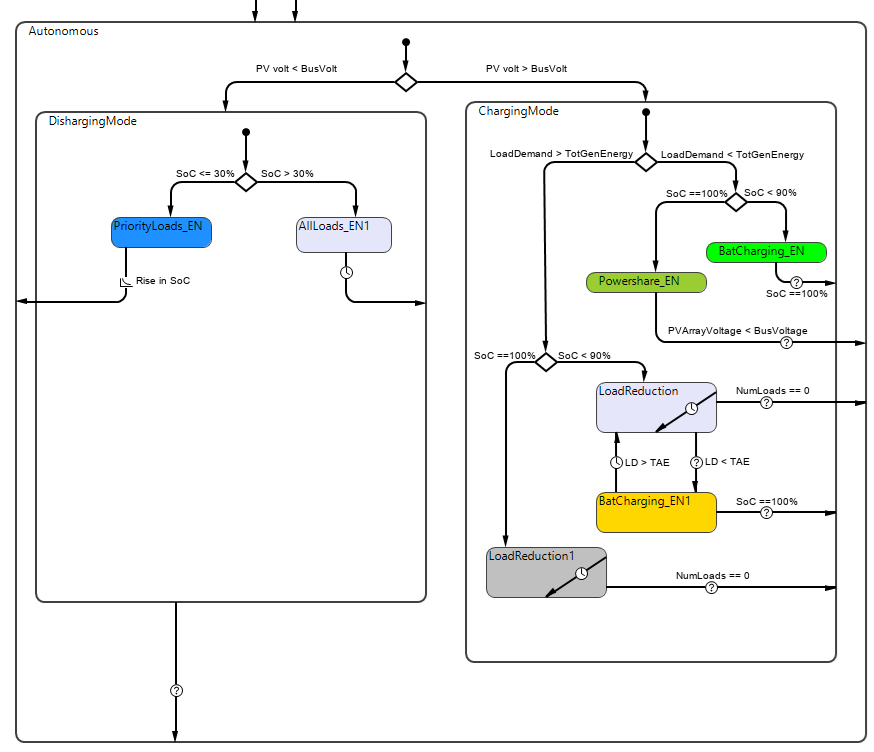
\includegraphics[totalheight=12cm]{Figures/opmod1 strategy.png}
	\caption{Operating mode 1 strategy}
	%	\label{fig:verticalcell}
\end{figure}
Figure 3.1 illustrates the control strategy for mode 2 operation, where the unit functions as a battery storage due to the availability of battery capacity. In this mode, priority is given to battery charging, ensuring that the load can continue to operate long after sunset. When there is insufficient energy from the grid to charge the battery and meet the load demand, the system activates the load reduction state.\par
\begin{figure}[H]
	\centering
	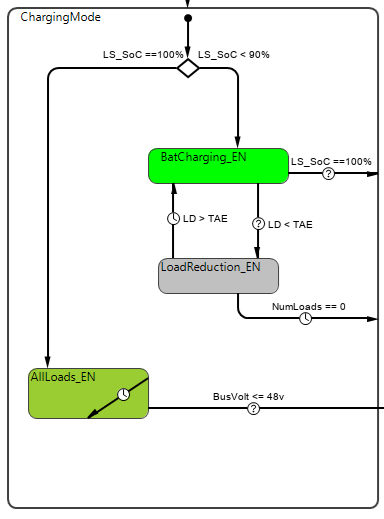
\includegraphics[totalheight=12cm]{Figures/opmod2 strategy.png}
	\caption{Operating mode 2 strategy}
	%	\label{fig:verticalcell}
\end{figure}
Mode 3 characterizes a residential unit that generates power but lacks a storage system. Figure 3.3 illustrates the state machine for this unit. The system enters a power-sharing state when the PV array generates sufficient power to meet the local demand. The State of Charge (SoC) of distributed energy sources can be estimated with reasonable accuracy using the filtered terminal voltage method proposed in in \cite{40}. This estimation allows the residential unit to contribute energy to charge the Energy Storage System (ESS) on the grid.\par
\begin{figure}[H]
	\centering
	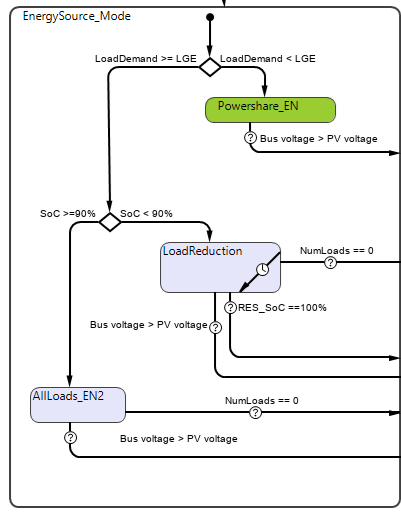
\includegraphics[totalheight=12cm]{Figures/opmod3 strategy.png}
	\caption{Operating mode 3 strategy}
	%	\label{fig:verticalcell}
\end{figure}
The control strategy for modes without any energy source or battery storage is simple: load reduction is triggered when the solar farm State of Charge falls below 10\%. This system solely relies on external power sources.\par
\begin{figure}[H]
	\centering
	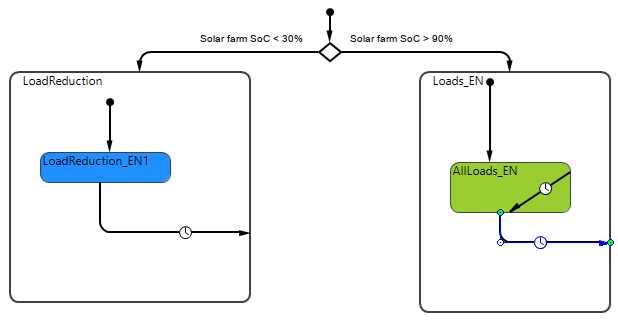
\includegraphics[totalheight=8cm]{Figures/opmod4 strategy.png}
	\caption{Operating mode 4 strategy}
	%	\label{fig:verticalcell}
\end{figure}
\section{Conclusion}
In this chapter, we conducted a feasibility study of the Energy Management System (EMS) and the DC Microgrid (MG) as a whole. Several authors have demonstrated the feasibility of DC MGs for residential use, with the EMS serving as an enhancement to the DC MG. We also explored power balancing and control strategies for managing units connected to the MG. The MG can be configured to operate in both centralized and decentralized (autonomous) modes. Additionally, state charts for the units were developed.\par

